\chapter{Verwendete Technologien}\label{cha:used-technologies}

\section{ESP-IDF Toolchain}\label{sec:esp-idf-toolchain}

Um die Toolchain verwenden zu können muss man sich in einem ESP-IDF Projektverzeichnis befinden. Hier kann ist es möglich, mit folgendem Befehl, den ESP zu konfigurieren:

\begin{verbatim}
    idf.py menuconfig
\end{verbatim}

Dieser Befehl sollte zu folgendem Menü führen:
\begin{figure}[H]
    \begin{center}
        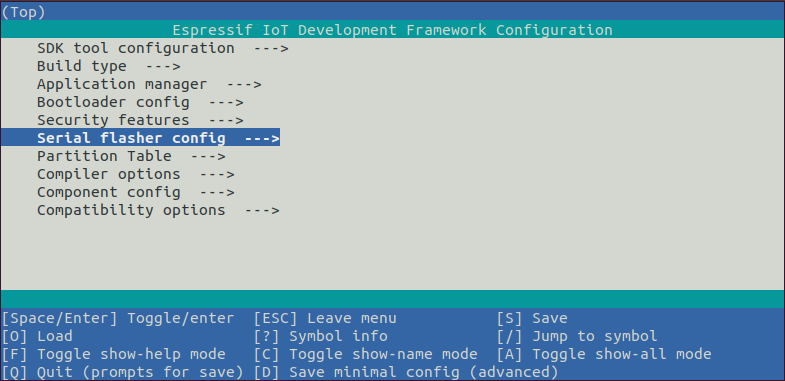
\includegraphics[scale=0.5]{images/menuconfig.png}
        \caption{menuconfig \cite{menuconfig_picture}}
    \end{center}
\end{figure}
\pagebreak
Dieses Menü wird verwendet um Projekt spezifische Variablen zu setzten. Wie zum Beispiel:
\begin{itemize}
    \item Netzwerkname
    \item Netzwerkpasswort
    \item Takt des Prozessors
    \item Parition Table Variante
    \item \dots und viele mehr
\end{itemize}

Weiters ist hier zu beachten, dass, wenn man auf einem Dual-Core ESP arbeiten sollte zuerst auf den Single-Core Modus umstellen sollte, bevor man die fertigen Beispiele von Espressif ausprobiert.

Ist das Projekt richtig konfiguriert kann man es mit dem folgendem Befehl builden:
\begin{verbatim}
    idf.py build
\end{verbatim}

Mit diesem Befehl wird die Anwendung kompiliert und der Bootloader und der Partition Table wird erstellt.

Sollten beim Kompilieren Fehler auftreten, so werden diese nun in der Konsole ausgegeben. Ist dies nicht der Fall kann das Program mit diesem Befehl auf den ESP geflashed werden:
\begin{verbatim}
    idf.py flash
\end{verbatim}

Sollte es ein Problem beim flashen geben, liegt dies häufig an einem kaputten USB-Kabel.

Um nun überprüfen zu können, ob das Program so läuft, wie es soll, kann man mit:
\begin{verbatim}
    idf.py monitor
\end{verbatim}
den IDF Monitor (\ref{sec:monitor}) starten.

Es ist auch möglich ein einem einzigen Befehlt das Program zu builden, zu flashen und upzuloaden:
\begin{verbatim}
    idf.py flash monitor
\end{verbatim}

\subsubsection{IDF Monitor}\label{sec:monitor}
Der IDF-Monitor ist ein serielles Terminalprogramm, das serielle Daten zum und vom seriellen Anschluss des Zielgeräts weiterleitet.

% TODO: write about esp tasks and other functionality we used
% Task
% Menuconfig (wie man ui benutzt und wie eine .projbuild datei funktioniert)
% Wie flashed man
% Was ist ein monitor
% Mögliche Probleme (falscher port etc, wie kann man diese lösen)

\section{Nodejs}\label{sec:nodejs}

Nodejs ist eine Laufzeit die auf der Javascript Engine von Chrome aufbaut. Nodejs wurde für das Backend des OTA Servers verwendet.

\subsection{Warum Nodejs?}

Java EE wurde hier nur als ein Beispiel gewählt. Folgendes gilt für jedes Framework das HTTP requests wie JavaEE behandelt. 
Bei der Überlegung welche Sprache bzw. welches Framework für das backend gewählt wird, war die Entscheidung sehr leicht.
Die Anforderungen des OTA Servers sind sehr einfach. Der Server dient nur zur Bereitstellung der Firmwares und beschreibende Informationen über die Firmwares selber.
Da dies nicht CPU intensiv ist sondern I/O intensiv, wurde in diesem Fall Nodejs gewählt.

\subsection{Event Loop}

\subsubsection{Was ist der Event Loop?}

Nodejs selber ist single-threaded deswegen ist der Event Loop einer der wichtigsten Bestandteile von Nodejs.
Der Event Loop erlaubt es nicht-blockenede I/O Operationen durchzuführen. Dies passiert durch die Abladung auf den Kernel von so vielen Operationen wie möglich.
\newline
\newline
Die meisten modernen Kernels sind multi-threaded. Das bedeutet, dass sie mehrere Operationen im Hintergrund unterstützen.

\subsubsection{Wie funktioniert der Event Loop?}

\begin{figure}[H]
    \begin{center}
        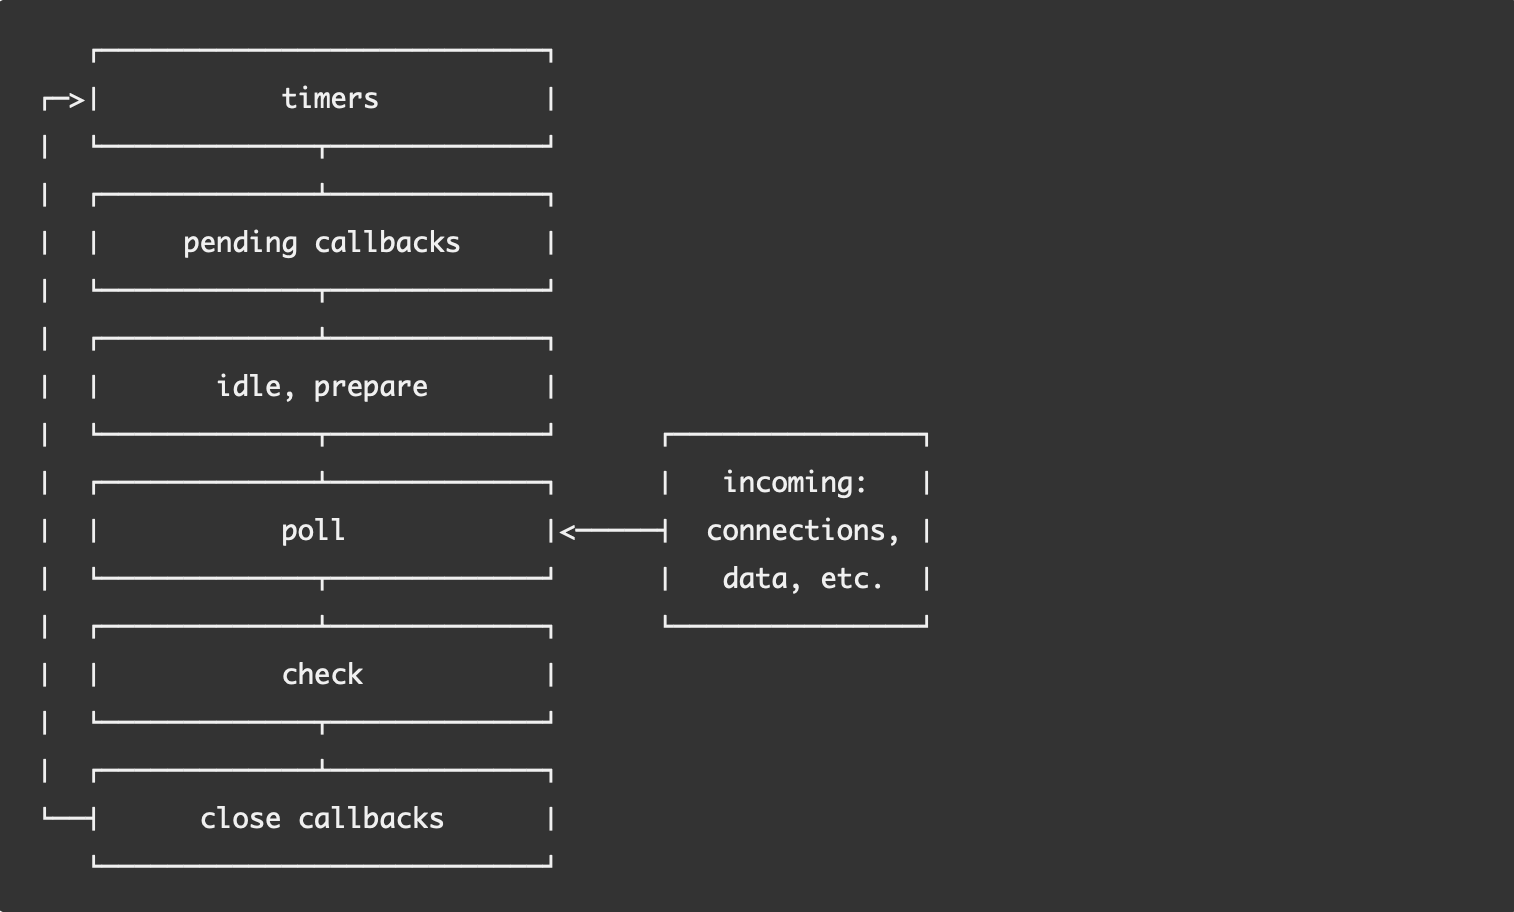
\includegraphics[scale=0.5]{images/nodejs_event_loop.png}
        \caption{Nodejs Event Loop \cite{nodejs_event_loop}}
    \end{center}
\end{figure}

Jeder Block im obigen Bild wird als Phase bezeichnet.
Jede Phase verfügt über eine First-In-First-Out-Warteschlange (FIFO-Warteschlange) mit auszuführenden Rückrufen. 
Während jede Phase auf ihre Weise etwas Besonderes ist, führt sie im Allgemeinen,
wenn die Ereignisschleife in eine bestimmte Phase eintritt, alle für diese Phase spezifischen Operationen aus und führt dann Rückrufe in der Warteschlange dieser Phase aus, 
bis die Warteschlange erschöpft ist oder die maximale Anzahl von Rückrufen ausgeführt hat. 
Wenn die Warteschlange erschöpft ist oder das Rückruflimit erreicht ist, wechselt die Ereignisschleife zur nächsten Phase und so weiter.
\newline
\newline
Da für jeden dieser Vorgänge möglicherweise mehr Vorgänge geplant werden und neue Ereignisse, 
die in der Abfragephase verarbeitet wurden, vom Kernel in die Warteschlange gestellt werden, 
können Abrufereignisse in die Warteschlange gestellt werden, während Abrufereignisse verarbeitet werden. 
Infolgedessen können lange laufende Rückrufe dazu führen, dass die Abfragephase viel länger als der Schwellenwert eines Timers läuft. 

\subsubsection{Phasen}

\begin{itemize}
    \item \textbf{timers:} In dieser Phase werden von setTimeout () und setInterval () geplante Rückrufe ausgeführt.
    \item \textbf{pending callbacks:} führt I/O Callbacks aus, die auf die nächste Iteration verschoben werden
    \item \textbf{idle, prepare:} wird nur intern verwendet
    \item \textbf{poll:} neue I/O Events abrufen; I/O bezogene Callbacks ausführen (fast alle mit Ausnahme von schließ Callbacks, die von Timers geplant werden, und setImmediate ()); Der Knoten wird hier gegebenenfalls blockiert
    \item \textbf{check:} setImmediate() Callbacks werden hier ausgeführt
    \item \textbf{close callbacks:} schließ Callbacks werden ausgeführt
\end{itemize}

Zwischen jedem Durchlauf des Event Loops prüft Nodejs, ob es auf asynchrone I/O oder Timer wartet, und fährt sauber herunter, wenn keine vorhanden sind.

\cite[Zitiert von der offizielen Nodejs Website]{nodejs_event_loop_how_does_it_work}

\section{Platform IO}\label{sec:platformio}

PlatformIO ist ein fortschrittliches und äußerst vielseitiges Ökosystem für die IoT-Entwicklung, das eine IDE, ein Build-System, einen Unified Debugger und einen Bibliotheksmanager umfasst. Es bietet Unterstützung für mehr als 550 Entwicklungsboards, mehr als 25 Entwicklungsplattformen und mehr als 10 nützliche Frameworks. Die PlatformIO IDE ist ein plattformübergreifendes Dienstprogramm für die schnelle berufliche Weiterentwicklung mit integriertem C / C++ - Intelligent Code Completion, Smart Code Linter und erweitertem Serial Port Monitor. PlatformIO kann auch in die gängigen IDEs und kontinuierlichen Integrationssysteme integriert werden, um die Zeit für die Bereitstellung von IoT-Anwendungen zu verkürzen.\cite{platformio_about_us}

PlatformIO ist in reinem Python geschrieben und hängt nicht von zusätzlichen Bibliotheken / Tools eines Betriebssystems ab. So kann man mit PlatformIO auf Windows, Macintosh und Linux arbeiten.

\section{ESP IDF Toolchain}\label{sec:platformio}

% TODO: Start

\section{Docker}\label{sec:docker}

% TODO: Start

\section{Docker Compose}\label{sec:docker-compose}

Docker-compose ist ein Tool zum Definieren und Ausführen von Docker-Anwendungen mit mehreren Containern. Mit Compose verwenden Sie eine YAML-Datei, um die Dienste Ihrer Anwendung zu konfigurieren. Anschließend erstellen und starten Sie mit einem einzigen Befehl alle Dienste in Ihrer Konfiguration. \cite{docker_compose_description}

\subsection{Docker Compose Beispiel}

\begin{figure}[H]
    \begin{center}
        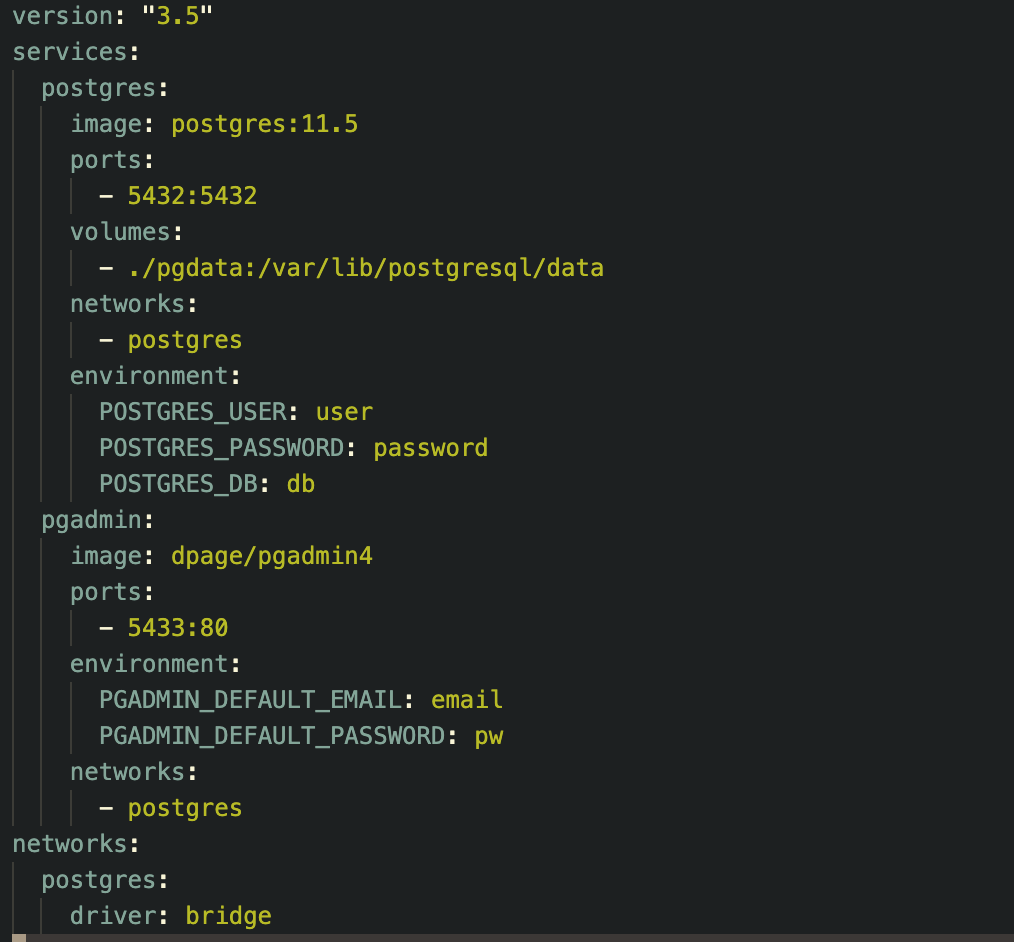
\includegraphics[scale=0.8]{images/docker_compose_example.png}
        \caption{Docker Compose Beispiel (Quelle: eigene Darstellung)}
    \end{center}
\end{figure}

In der obigen Abbildung kann man das docker-compose.yml file von dem OTA Server sehen.

Die Struktur eines docker-compose files ist im Normalfall immer gleich. Am Anfang definiert man welche Version des Standards man verwendet und anschließend die verschiedenen Dienste. Der OTA Server benötigt nur 2 Dienste:

\begin{enumerate}
    \item Postgres
    \item PgAdmin4
\end{enumerate}

In diesem Beispiel wird das Netzwerk explizit erstellt. Es ist auch möglich das Netwerk implizit zu erstellen, indem man den networks Bereich von ganz unten entfernt.

\subsubsection{Postgres}

Datenbank für die Speicherung von den Informationen über die verschieden Firmwares die gerade auf dem Server hochgeladen sind.

Die Datenbank braucht irgendeinen Weg um mit der Außenwelt kommunizieren zu können, deswegen wird der interne Port 5432 auf den externen Port 5432 geleitet.

Damit die Absicherung der Datenbank leicht verläuft wird ein Volume für die Datenbank erstellt, worin sich die Daten der Datenbank befinden. In dieser docker-compose Datei wird das Volume implizit erstellt. 

Man kann es auch explizit erstellen wie folgt:

\begin{verbatim}
    volumes:
        pgdata:
\end{verbatim}

Mit den Umgebungsvariablen kann man die Standardwerte überschreiben. Die Datenbank hat in der obigen Abbildung den Benutzer \textit{user} mit dem Passwort \textit{password} und der default Datenbank \textit{db}.

\subsubsection{PgAdmin4}

PgAdmin4 ist eine web-basierte Benutzeroberfläche für Postgres.

Sie ist die PhpMyAdmin Oberfläche in der postgres Welt.

Die Software binded automatisch auf den Port 80, was für Entwicklungszwecke sehr unpraktisch ist, da Port 80 auf Ubuntu zum Beispiel Adminrechte benötigt. Deswegen wird der interne Port 80 auf den externen Port 5433 umgeleitet.

Mit den Umgebungsvariablen \textit{PGADMIN\_DEFAULT\_EMAIL} und 
\textit{PGADMIN\_DEFAULT\_PASSWORD} werden die default Logindaten für PgAdmin4 definiert. 

\section{ESP IDF Utility lib}\label{sec:esp-idf-utility-lib}

% TODO: Start
